%!TEX root = ../my_thesis.tex

\chapter{Les codes polaires}

Résumé

\vspace*{\fill}
\minitocTITI
\vspace*{\fill}

% \subsection*{Introduction}

\section{Le principe et la construction des codes polaires}

\subsection{La chaîne de communication numérique}
\label{subsec:contexte}


\begin{figure}[t]
\centering
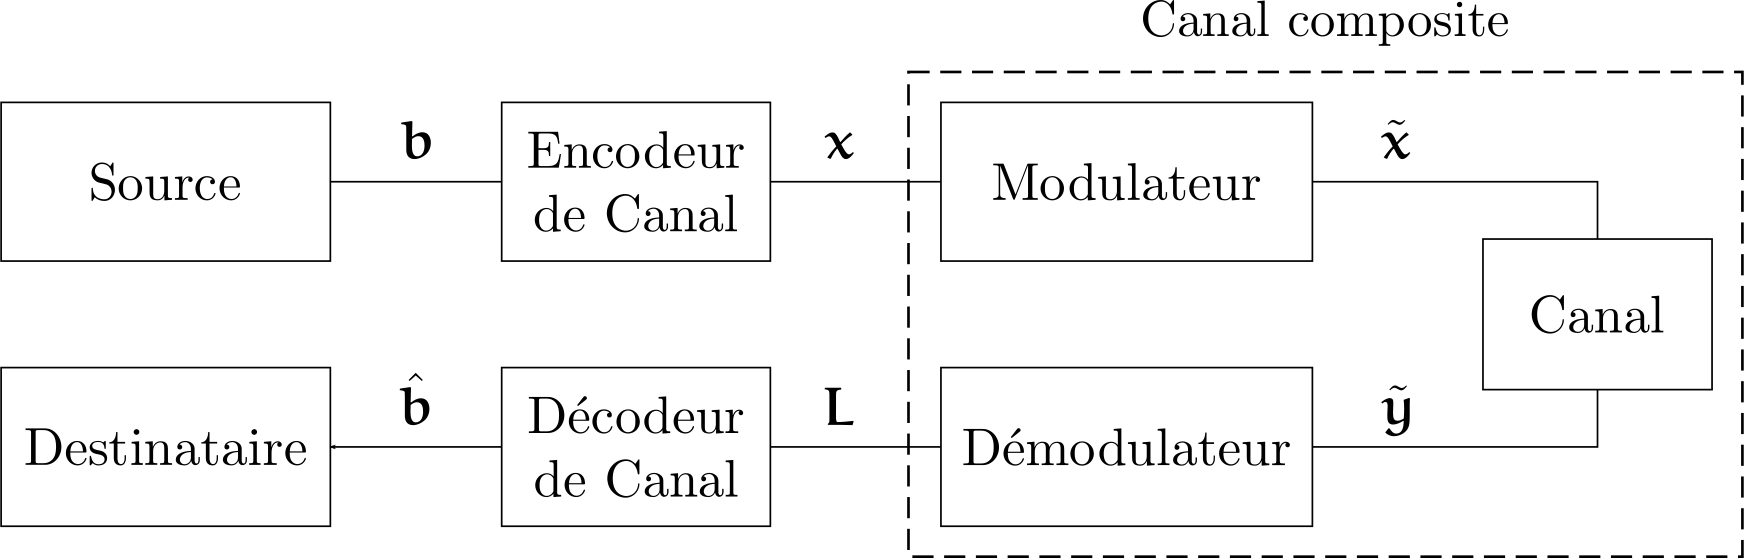
\includegraphics[width=0.8\textwidth]{main/ch1_fig/chaine_com}
\caption{Modèle simplifié d'une chaîne de communication}
\label{fig:chaine_com}
\end{figure}
Une chaîne de communication numérique telle que conceptualisée par Claude Shannon \cite{shannon_mathematical_2001} est représentée en Figure~\ref{fig:chaine_com}.
Elle représente les principales étapes de la transmission de données numériques depuis une \textbf{source} vers un \textbf{destinataire} à travers un \textbf{canal} de transmission.
Ce dernier est le support sur lequel transite l'information. Lors de communications sans fil, il s'agit de l'ensemble constitué des antennes d'émission et de réception et de l'espace les séparant. Or les grandeurs physiques associées à ce canal sont continues tandis que les données à transmettre sont constituées de bits, donc discrètes. Le \textbf{modulateur} transforme ce flux binaire en signaux physiques transmissibles par le canal. Si l'on considère toujours les communications sans fils, le modulateur transforme les séquences de bits en formes d'ondes. Au sein du canal de communication, les signaux subissent de nombreuses perturbations comme le bruit thermique des composants électroniques de la chaîne de transmission ou encore les interférences causées par d'autres utilisateurs du canal. Le démodulateur effectue la fonction duale du modulateur, il convertit les signaux physiques en données binaires. Si les perturbations du canal sont trop fortes, il est possible que le modulateur génère une estimation erronée du bit transmis. Ceci est un problème, puisque le but de la chaîne de transmission est de transmettre au destinataire l'exacte réplique de la \textbf{séquence d'information}, $\mathbold{b}$ émise par la source. Lorsque l'information reçue et l'information émise diffèrent, il y a erreur de transmission. La qualité de la chaîne de transmission est souvent mesurée par son taux d'erreur binaire (BER), qui correspond à la proportion d'erreurs binaires par rapport au nombre total de bits transmis.

L'ajout d'un encodeur et d'un décodeur canal dans la chaîne de transmission est un moyen efficace de réduire ce taux d'erreur. Dans le cas des codes en blocs étudiés dans ce manuscrit, l'encodeur transforme une séquence d'information $\mathbold{b}$ de $K$ bits en un \textbf{mot de code} $\mathbold{x}$ de $N$ bits. La taille du mot de code, en nombre de bits, est supérieure à la taille de la séquence d'informations afin d'ajouter de la redondance au message transmis: le rendement du code $R=K/N$ est inférieur à $1$. Cette redondance est utilisée par le décodeur de canal, ou parfois le couple démodulateur - décodeur canal, afin d'améliorer l'estimation du message transmis et donc de réduire le taux d'erreur binaire de la chaîne de transmission. Dans ce manuscrit, le décodeur de canal est découplé du démodulateur. L'ensemble modulateur - canal - démodulateur peut être considéré comme une seule entité indépendante dont l'entrée est constituée du mot de code $\mathbold{x}$ et la sortie d'une séquence d'estimation de $\mathbold{x}$ notée $\mathbold{L}$. Cet ensemble est appelé canal composite.

\subsection{Le canal composite}
\label{subsec:canal}

Un seul et unique modèle de canal composite sera considéré tout au long de ce manuscrit. Il est constitué d'un modulateur à changement de phase binaire (BPSK) qui associe aux valeurs binaires d'entrée $x\in\{0,1\}$ les valeurs réelles $\tilde{x}\in\{-1,1\}$, respectivement.

Le canal composite considéré utilise un canal à bruit blanc additif gaussien à entrée binaire (BI-AWGNC : Binary Input - Additive White Gaussian Noise Channel) tel que défini dans \cite[Section~1.5.1.3]{ryan2009channel}. Ce modèle est le plus utilisé pour caractériser les performances des codes correcteurs d'erreur. Il consiste en l'addition aux données de sortie du modulateur $\mathbold{\tilde{x}}$ d'une variable aléatoire à valeurs réelles ayant une distribution gaussienne centrée en $0$ et de densité spectrale $N_0$. Afin d'évaluer les performances de correction des codes correcteurs d'erreurs, les taux d'erreurs seront souvent rapportés à cette densité spectrale, ou plus précisément au \textbf{rapport signal à bruit} (SNR), noté $E_b/N_0$, où $E_b=\frac{\mathbb{E}(\hat{x}^2)}{R}$ est l'énergie moyenne par bit d'information.

Les estimations en sortie du démodulateur sont données sous la forme de rapport de vraisemblance logarithmique (LLR : Logarithmical Likelihood Ratio). Leur signe détermine pour chaque donnée $\hat{y}_i \in \mathbold{\hat{y}}$ la valeur binaire d'entrée $\hat{x}_i \in \mathbold{\hat{x}}$ la plus probable. Leur valeur absolue le degré de fiabilité de l'information. Des détails sur le modèle de canal et la définition des LLRs sont donnés en Annexe \ref{append:decoding_nodes} et leur définition mathématique est la suivante : 

\begin{equation*}
  L_i = \log\left(\dfrac{P_r(y_i | x_i = 0)}{P_r(y_i | x_i = 1)}\right)
\end{equation*}


\subsection{L'encodage de codes polaires}
Les codes polaires \cite{arikan_channel_2009} sont des codes en blocs linéaires \cite{morelos-zaragoza_art_2006}. Soient les ensembles $\mathbb{B}^n = \{0,1\}^n$, et une matrice $G \in \mathbb{B}^K \times \mathbb{B}^N$, l'encodage d'un code en blocs linéaire est une application linéaire injective de $\mathbb{B}^K$ vers $\mathbb{B}^N$ qui à un élément $\mathbold{b} \in \mathbb{B}^K$ associe un élément $\mathbold{x} \in \mathbb{B}^N$ tel que $x=\mathbold{b}G$. Les codes polaires peuvent ainsi être défini comme l'ensemble des codes en blocs linéaires ayant une matrice génératrice avec une forme particulière.

La matrice génératrice d'un code polaire est elle-même produit de deux matrices $E \in (\mathbb{B}^K \times \mathbb{B}^N)$ et $F^{\otimes n}\in (\mathbb{B}^N)^2$, $G=EF^{\otimes n}$. La multiplication par la matrice $E$ correspond à l'introduction de "bits gelés", dont la valeur est $0$, à la séquence d'information $\mb{b}$. Le résultat de l'opération $\mathbold{u} = E\mathbold{b}$ est constitué de $K$ bits $b_i \in \mathbold{b}$ et de $N-K$ bits gelés. Les positions respectives des bits d'informations et des bits gelés sont liées au phénomène de polarisation décrit dans la section suivante. Ces positions sont déterminantes quant au pouvoir de correction du code.

La matrice $F^{\otimes n}$, où $N=2^n$, est la n-ième puissance de Kronecker du noyau $F=\left[\begin{smallmatrix} 1 & 0 \\ 1 & 1\end{smallmatrix}\right]$. On peut définir $F^{\otimes n}$ récursivement : $F^{\otimes 1} = F$ et $\forall {n \geq 1}\text{ , }{F^{\otimes n + 1}=\left[\begin{smallmatrix} F^{\otimes n} & 0_n \\ F^{\otimes n} & F^{\otimes n}\end{smallmatrix}\right]}$ avec $0_n \in \mathbb{B}^N$ une matrice nulle. La représentation sous forme de \textit{factor graph}, en figure \ref{fig:encodage}, est une représentation graphique du processus d'encodage de codes polaires où les symboles $\oplus$ correspondent à des opération \textit{OU-exclusif}. 

\begin{figure}[t]
\centering
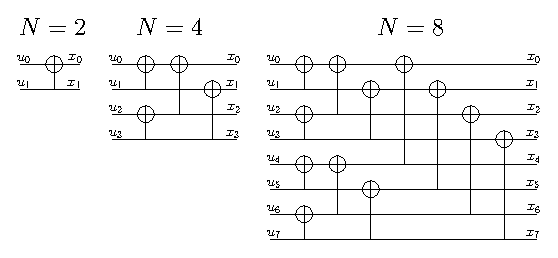
\includegraphics[width=0.5\textwidth]{main/ch1_fig/Graph_N_rec}
\caption{Représentation en \textit{factor graph} de l'encodage de codes polaires}
\label{fig:encodage}
\end{figure}

Le processus d'encodage peut également être modifié pour rendre le code systématique. Un code correcteur d'erreur est dit systématique si les bits de la séquence d'information sont présents dans le mot de code. Pour ce faire, il faut modifier la matrice d'encodage comme démontré dans \cite{arikan_systematic_2011} : $G_{sys}=EF^{\otimes n}EF^{\otimes n}$. La représentation en \textit{factor graph} de cette matrice est donnée en Figure \ref{fig:sys}. Lorsque cette matrice d'encodage est utilisée, les bits de la séquence d'information $\mb{b}$ se trouvent dans le mot de code $\mb{x}$, car $\mb{x}=\mb{b}G_{sys}$, alors $\mb{b}=E^{-1}\mb{x}$ .

\begin{figure}[t]
\centering
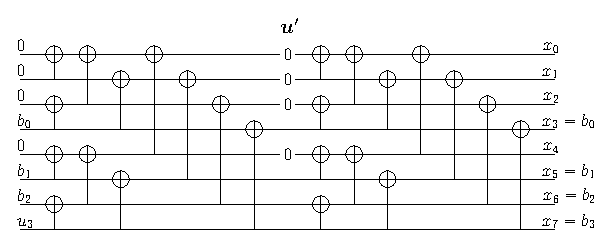
\includegraphics[width=0.7\textwidth]{main/ch1_fig/Graph_N_sys}
\caption{Encodage systématique}
\label{fig:sys}
\end{figure}

\subsection{Le phénomène de polarisation}
\label{subsec:polarisation}
La spécificité des codes polaires est liée au phénomène de polarisation. L'ensemble constitué de l'encodeur polaire, du canal composite et du décodeur polaire peut être modélisé comme un ensemble de canaux de transmission qui chacun transmet un bit. Le terme \og polarisation \fg exprime le fait que ces $N$ canaux ont tendance à se diviser en deux groupes. Un groupe de canaux très fiables, avec une probabilité d'erreur faible, et un groupe de canaux peu fiables, à probabilité d'erreur forte.
Il est possible de montrer que la proportion de canaux très fiable, pour un rendement de code donné, tend vers la capacité du canal tel que définie dans la théorie de l'information \cite{shannon_mathematical_2001} lorsque la taille du mot de code $N$ tend vers l'infini.
Lors de l'étape d'encodage, les bits d'informations seront attribués aux canaux fiables et les bits dits gelés, dont la valeur est connue à priori, sont attribués aux canaux peu fiables. La transformation en produit de Kronecker étant commune à tout les codes polaires, la construction d'un code polaire consiste uniquement à déterminer la position des bits gelés dans le vecteur $\mathbold{u}$ pour une taille de code donnée. La construction des codes polaires est déterminante quant à leur pouvoir de correction. La méthode de détermination des positions des bits gelés est donné dans \cite{arikan_channel_2009} seulement pour les canaux à effacement. Pour le canal AWGN, les premières tentatives furent données dans \cite{mori_performance_2009,mori_properties_2010} mais leur complexités calculatoires sont significatives. Des méthodes simplifiées, utilisées dans la pratique, ont été proposées dans \cite{tal_how_2013,trifonov_efficient_2012,trifonov_randomized_2018} pour le canal AWGN. La valeur des bits gelés, dans la plupart des cas, est 0. Toutefois, certains travaux \cite{trifonov_polar_2016,trifonov_randomized_2017} montrent que de meilleures performances de décodage peuvent être atteintes en assignant des valeurs dynamiques à ces bits gelés. Dans l'ensemble des simulations et des explications contenues dans ce manuscrit, il est cependant considéré que la valeur des bits gelés est 0.

\section{Les algorithmes de décodage de codes polaires}

Deux algorithmes de décodage ont été proposés dès l'invention des codes polaires \cite{arikan_channel_2009}. L'algorithme de décodage appelé Annulation Successive (SC) est un algorithme de décodage à sortie dure : les données de sortie sont des bits. L'algorithme de décodage par propagation de croyance (BP) est au contraire un algorithme de décodage itératif à sortie souple, dont les données de sortie sont des estimations représentée typiquement par des LLRs. De nombreuses variantes de ces algorithmes ont ensuite été proposées pour en améliorer les performances de corrections. Les algorithmes Annulation Successive par Liste (SCL) \cite{tal_list_2011}, Annulation Successive "Flip" (SCF) \cite{afisiadis_low-complexity_2014}, Annulation Successive par Pile (SCS) \cite{niu_stack_2012} sont des évolutions de l'algorithme SC. Au contraire, l'algorithme appelé Annulation Souple (SCAN) \cite{fayyaz_low-complexity_2014} peut être vu comme une combinaison des algorithmes SC et BP. Chacun de ces algorithmes est décrit dans cette section.

\subsection{L'algorithme de décodage par Annulation Successive}

% Ajouter channel LLRs à la racine
\subsubsection{Les fonctions élémentaires}

\begin{figure}[t]
  \renewcommand*\thesubfigure{\arabic{subfigure}} 
  \centering
  \subfloat[][Channel LLRs]{\includegraphics[width=.26\textwidth]{main/ch1_fig/sc_graph_1}}\quad\quad
  \subfloat[][$f$ function]{\includegraphics[width=.18\textwidth]{main/ch1_fig/sc_graph_2}}\quad\quad
  \subfloat[][$\texttt{R0}$ function]{\includegraphics[width=.2\textwidth]{main/ch1_fig/sc_graph_3}}\\
  \subfloat[][$g$ function]{\includegraphics[width=.18\textwidth]{main/ch1_fig/sc_graph_4}}\quad\quad
  \subfloat[][$\texttt{R1}$ function]{\includegraphics[width=.2\textwidth]{main/ch1_fig/sc_graph_5}}\quad\quad
  \subfloat[][$h$ function]{\includegraphics[width=.18\textwidth]{main/ch1_fig/sc_graph_6}}
  \caption{Fonctions élémentaires et séquencement du décodage SC du noyau $N=2$}
  \label{fig:sc_steps}
\end{figure}

% Expliciter notation (N,K)
% Mettre cohérence dans numérotation des couches (0 = racine)

%
Les étapes du décodage du \noeud élémentaire de taille 2 sont représentées en Figure~\ref{fig:sc_steps}.
Les données d'entrée des algorithmes de décodages présentés ici sont des LLRs, contenus dans le vecteur $\mathbold{L}$ de taille $N$, sorti du canal composite.
En effet, si les premières descriptions de l'algorithme SC utilisaient directement les probabilités ou bien les rapports de vraisemblance (LR : Likelihood Ratio), des versions utilisant les LLRs ont systématiquement été proposées, comme pour l'algorithme SC \cite{leroux_hardware_2011} et l'algorithme SCL \cite{balatsoukas-stimming_llr-based_2015}.
Les données de sorties du décodeur sont quant à elles des bits contenus dans le vecteur $\mathbold{\hat{b}}$ de taille $K$.
Au cours du décodage de codes polaires, les deux formats de données,  les LLRs d'une part, et les sommes partielles (PS : Partial Sums) qui sont des valeurs binaires, sont utilisés. 
Huit variables sont nécessaires pour le décodage du noyau élémentaire de taille 2 : 4 LLRs notés $L_{i,j}$ et 4 sommes partielles notées $s{i,j}$. Les deux types de données apparaissent dans la Figure \ref{fig:sc_steps} qui représentent les différentes étapes de l'algorithme de décodage SC, sous forme de \textit{factor graph}.
La première étape (1) du décodage est le chargement des LLRs du canal $L$ : les LLRs $L_{0,0}$ et $L_{1,0}$ prennent la valeur des LLRs du canal. Les LLRs et les sommes partielles de chaque \noeud de l'arbre sont ensuite calculées par l'intermédiaire des opérations $f$, \texttt{R0}, $g$, \texttt{R1} et $h$ symbolisées dans la Figure~\ref{fig:sc_steps} par des flèches. Elles correspondent aux équations \ref{eq:sc} :
\begin{eqnarray}
  \begin{array}{l c l}
    f(L_a,L_b) &=& \text{sign}(L_a.L_b).\min(|L_a|,|L_b|)\\
    g(L_a,L_b,\hat{s}_a)&=&(1-2\hat{s}_a)L_a+L_b\\
    h(\hat{s}_a,\hat{s}_b)&=& (\hat{s}_{a} \oplus \hat{s}_{b}, \hat{s}_{b})\\
    \texttt{R0}(L_a) &=& 0 \\
    \texttt{R1}(L_a) &=&  \left\{\begin{array}{l c l} 0 \text{ si } L_a \geq 0 \\ 1 \text{ si } L_a < 0 \end{array}\right.
  \end{array}
  \label{eq:sc}
\end{eqnarray}
La fonction $f$ est appliquée dans l'étape (2) et permet le calcul de $L_{0,1}$.
L'étape (3) est l'application de la fonction \texttt{R0} sur le \noeud supérieur. 
La fonction \texttt{R0} est appliquée dans l'hypothèse où le bit encodé $u_0$ en Figure \ref{fig:encodage} est un bit gelé.
La fonction $g$ permet ensuite, en étape (4), le calcul de $L_{1,1}$.
L'étape (5) est le calcul de $s_{1,1}$ par l'opération \texttt{R1} correspondant à un bit d'information. 
Cette opération est un seuillage du LLR pour obtenir la somme partielle.
Pour rappel, dans la représentation en LLR, le signe correspond à la décision dure : bit égal à 0 pour un LLR positif, bit égal à 1 pour un LLR négatif. 
La valeur absolue informe sur la fiabilité de cette décision.
Lorsque le seuillage est réalisé, l'information de fiabilité est perdue.
Après le décodage de la somme partielle $s_{1,1}$, la fonction $h$ est appliquée afin de propager les sommes partielles, en étape (6).


\subsubsection{L'arbre de décodage}
\begin{figure}[t]
\centering
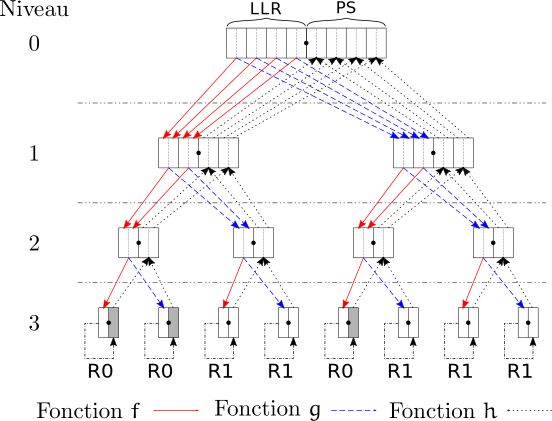
\includegraphics[width=0.55\textwidth]{main/ch1_fig/sc}
\caption{Arbre de décodage SC}
\label{fig:sc}
\end{figure}
\begin{figure}[t]
\centering
\includegraphics[width=0.5\textwidth]{main/ch1_fig/seq_sc}
\caption{Séquencement du décodage SC d'un code polaire de taille $N=4$.}
\label{fig:seq_sc}
\end{figure}
% mettre en évidence qu'on décode bit par bit, sera utile pour sc list
% introduire termes rendement 1 / rendement 0
% sommes partielles termes non introduit
% vérifier que n est introduit
Lorsque $N$ augmente, il est plus commode d'utiliser la représentation en arbre, comme montré en Figure~\ref{fig:sc}, où $N=8$.
Les données sont organisées en arbre binaire sur $log_2(N) + 1$ \textbf{couches}. Dans notre cas donc, l'arbre possède quatre couches.
A chaque couche sont attribués un certain nombre de \textbf{\noeuds}.
La \textbf{racine} de l'arbre numérotée $0$ est constituée d'un seul \noeud.
La racine contient $N$ LLRs et $N$ sommes partielles.
En descendant dans l'arbre, à chaque couche, le nombre de \noeuds double, tandis que le nombre de LLRs et de sommes partielles de chaque \noeud et divisé par deux.
Les \textbf{feuilles} sont les \noeuds les plus bas de l'arbre.
Le traitement d'une feuille correspond à l'application des opérations \texttt{R0} et \texttt{R1}.
Chaque couche $d$ contient $2^d$ \noeuds constitués de $2^{n-d}$ LLRs et de $2^{n-d}$ sommes partielles, où $n=\log_2(N)$. 
La hauteur jusqu'à laquelle les sommes partielles sont propagées par la fonction $h$ dépend de l'index de la feuille qui vient d'être décodé.

Dans le cas d'un code non systématique, la séquence décodée $\hat{u}$ est composée des sommes partielles contenues dans les feuilles de l'arbre de décodage..
Lors d'un décodage non systématique, les sommes partielles contenues par les feuilles correspondent à la séquence décodée $\hat{u}$.
La Figure~\ref{fig:seq_sc} est une représentation plus synthétique de l'arbre de décodage.
Les opérations 12 et 13 dans la Figure \ref{fig:seq_sc} sont donc inutiles puisqu'elles servent seulement à calculer les sommes partielles du \noeud racine.
Par contre, dans le cas d'un code systématique, ce sont les sommes partielles du \noeud racine qui correspondent au mot de code décodé.
Le parcours de l'arbre est un parcours en profondeur.
La séquence d'application des différentes fonctions est explicitée dans la Figure~\ref{fig:seq_sc}, où chaque flèche représentant une fonction est numérotée dans l'ordre.



\subsubsection{Le parallélisme de l'algorithme}
\label{subsubsec:parallel}
Dans la Figure~\ref{fig:sc}, il apparaît que quatre fonctions $f$ sont appliquées sur le \noeud racine pour calculer les LLRs de la branche de gauche. Ces quatre fonctions sont indépendantes : leurs entrées et sorties sont disjointes. Par conséquence, elles peuvent être réalisées simultanément. Ce parallélisme existe pour chaque fonction $f$, $g$ et $h$ d'un \noeud donné. Ainsi, le niveau de parallélisme est différent selon la couche considérée et correspond à la taille du \noeud cible. Le parallélisme est donc plus grand en haut de l'arbre qu'en bas. Dans les implémentations logicielles ou matérielles de ces algorithme, ce parallélisme est utilisé pour réduire le temps de décodage et accélérer son débit. Lorsque ce parallélisme est utilisé, on parle de parallélisme \textit{intra-trame}. Un autre type de parallélisme existe et est appelé parallélisme \textit{inter-trame}. Il désigne la possibilité, dans les implémentations de codes correcteurs d'erreurs, de décoder plusieurs trames simultanément. Il possède le désavantage, contrairement au parallélisme \textit{intra-trame}, d'augmenter la latence du décodage.


\subsection{L'algorithme de décodage par Annulation Successive à Liste}
\subsubsection{L'algorithme}
L'algorithme de décodage par Annulation Successive Liste (SCL) est une évolution de l'algorithme SC \cite{tal_list_2011}. L'algorithme SC présente en effet des performances de correction médiocres pour des codes polaires de petite taille. Le SCL améliore ces performances substantiellement. Dans l'algorithme de décodage SC décrit précédemment, des décisions dure sont réalisées à chaque traitement d'une feuille correspondant à un bit d'information (fonction \texttt{R1}). Si une erreur est commise lors de ce seuillage, celle-ci est irréversible, et le décodage du mot de code est un échec. Le principe de l'algorithme de décodage par liste est de retarder la décision dure. Au lieu d'appliquer un seuillage sur la valeur du LLR, les deux possibilités de décodage sont considérées, et l'arbre de décodage, avec l'ensemble de ses LLRs et sommes partielles, est dupliqué. Cette opération est représentée dans la Figure~\ref{fig:scl}.

L'algorithme est représenté en cours de réalisation, à l'étape (i), au cours de laquelle la fonction $f$ est appliquée. L'étape suivante (i+1) consiste en la duplication de l'arbre de décodage afin de former deux chemins. Dans le premier, l'hypothèse est que $\hat{u}_2=0$, dans le deuxième, $\hat{u}_2=1$. Le décodage continue ainsi sur les deux arbres parallèlement : l'étape suivante (i+2) l'application de la fonction $g$. Ces deux arbres sont qualifiés de \textbf{chemins} de décodage. \`A chaque feuille de rendement 1, le même procédé est réalisé, doublant le nombre d'arbres décodés en parallèle comme en étape (i+3).

\begin{figure}[t]
\centering
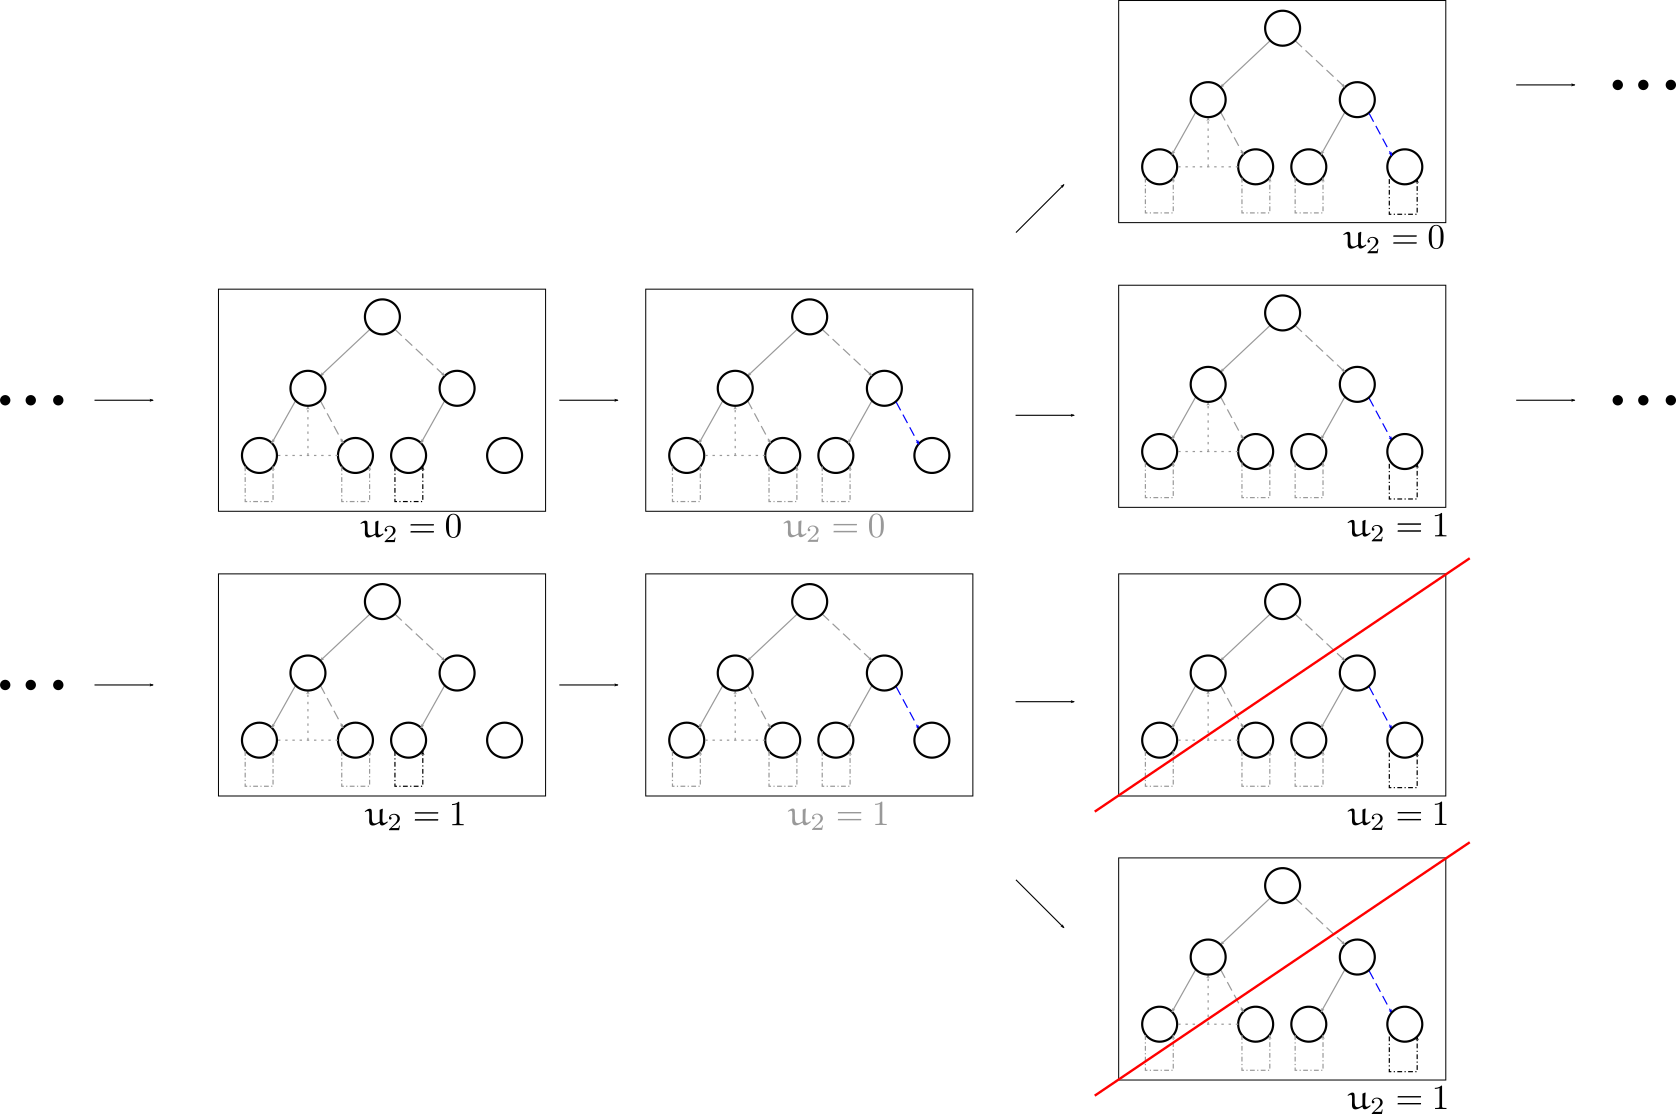
\includegraphics[width=1\textwidth]{main/ch1_fig/scl}
\caption{Duplication de l'arbre de décodage dans l'algorithme SCL.}
\label{fig:scl}
\end{figure}

Il n'est pas possible, en pratique, de dupliquer indéfiniment le nombre d'arbres de décodage, la mémoire nécessaire et le nombre de calcul devient vite insoutenable. Un nombre de chemins maximum $L$ est donc paramètre l'algorithme liste. Des La sélection des chemins qui seront conservés ou éliminés est réalisée grâce à une \textbf{métrique} $m^i_j$ associée à chaque chemin. Cette métrique est mise à jour à chaque traitement d'une feuille. Lors des autres étapes, par exemple l'application de la fonction $g$ en étape (i+2), les métriques sont inchangées, $m^{i+2}_j = m^{i+1}_j$. Le détail des calculs de métriques lors du traitement d'une feuille pour un décodage utilisant des LLRs est donné dans \cite{balatsoukas-stimming_llr-based_2015}. Lorsque la feuille est de rendement 0 si le LLR de la feuille est positif, la métrique est inchangée car l'estimation du LLR est en accord avec la valeur du bit gelé, 0. Si le LLR est négatif alors au contraire, la valeur absolue du LLR lui est ajoutée. Soit $i_0$ l'indice correspondant à une étape de traitement d'une feuille de rendement 0, et $L_j^{i_0}$ la valeur de son LLR, alors, pour un chemin donné d'indice $j$, 
\begin{equation*}
m^{i_0}_j=\left\{\begin{array}{l c l} m_j^{{i_0}-1} & \text{ si } L_j^{i_0} \geq 0 \\ m_j^{{i_0}-1} + |L_j^{i_0}| & \text{ si } L_j^{i_0} < 0 \end{array}\right.
\end{equation*}
Lorsque la feuille est de rendement 1, deux chemins sont créés, avec chacun une version différente du bit décodé. Le chemin créé dont la valeur du bit est en accord avec la valeur du LLR ne reçoit pas de pénalité. Au contraire, la métrique du deuxième chemin créé est accrue de la valeur du LLR. Soit $i_1$ l'étape de décodage d'une feuille de rendement 1,
\begin{equation*}
m^{i_1}_j=\left\{\begin{array}{l c l} m_j^{{i_1}-1}               & \text{ si } L^{i_1}_j \geq 0 \text{ et } \hat{u}^{i_1}_j = 0
                                   \\ m_j^{{i_1}-1} + |L^j_{i_1}| & \text{ si } L^{i_1}_j < 0    \text{ et } \hat{u}^{i_1}_j = 0
                                   \\ m_j^{{i_1}-1} + |L^j_{i_1}| & \text{ si } L^{i_1}_j \geq 0 \text{ et } \hat{u}^{i_1}_j = 1
                                   \\ m_j^{{i_1}-1}               & \text{ si } L^{i_1}_j < 0    \text{ et } \hat{u}^{i_1}_j = 1

                \end{array}\right.
\end{equation*}

Une fois ces calculs de métriques réalisés, on sélectionne les chemins à conserver. Si $L$ chemins étaient actifs au moment du traitement d'une feuille de rendement 1, alors $2L$ candidats sont générés, avec chacun une métrique associée. Seuls les $L$ candidats avec la métrique la plus faible sont conservés. Cette opération de sélection est représentée dans la Figure~\ref{fig:scl}. Lors de la dernière étape, à droite de la figure, les deux candidats du bas sont éliminés. L'hypothèse était donc que ces deux chemins avaient un métrique de valeur absolue supérieure aux métriques des deux candidat du haut. \`A la fin du parcours de l'arbre de décodage, $L$ chemins auront donc été conservés. Ces $L$ chemins correspondent à $L$ mots de codes possibles. Une sélection d'un seul candidat parmi les $L$ doit être effectuée. Dans la version originale de l'algorithme, le mot décodé associé au chemin ayant la métrique de valeur la plus faible à la fin du décodage est sélectionné comme étant la sortie de l'algorithme $\mathbold{\hat{b}}$.

% Insistier lourdement sur la signification de chaque terme : chemin, métrique, candidat

\subsubsection{Concaténation avec un CRC}

Les auteurs de \cite{tal_how_2013} ont proposé de concaténer un test de redondance cyclique (CRC) pour discriminer les différents candidats. L'encodage est représenté en Figure~\ref{fig:crc}. \`A la fin de l'algorithme de décodage, lorsque les $L$ mots de codes sont disponibles, un CRC est appliqué sur chacun d'entre eux. Si l'un d'entre eux vérifie le CRC, il est alors hautement probable qu'il soit le bon candidat.

\begin{figure}[t]
\centering
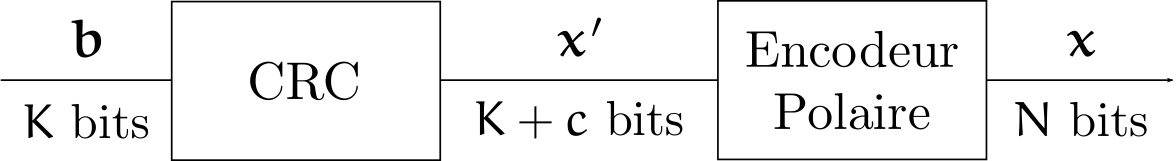
\includegraphics[width=0.6\textwidth]{main/ch1_fig/crc}
\caption{Concaténation avec un CRC.}
\label{fig:crc}
\end{figure}
\subsubsection{Les algorithmes de décodage adaptatifs}

%Citation
L'algorithme SCL adaptatif permet d'augmenter le débit des implémentations l'algorithme CA-SCL. La première étape est d'appliquer l'algorithme SC sur les LLRs de sortie du canal composite. Le test du CRC est alors réalisé. S'il est satisfait, le mot de code est considéré comme bon et le décodage est terminé. Dans le cas contraire, l'algorithme SCL est appliqué. Dans le cas de l'algorithme Partiellement Adaptatif (PA-SCL), l'algorithme est appliqué une seule fois avec comme taille de liste $L_{max}$. Dans le cas de l'algorithme Complètement Adaptatif (FA-SCL), après la première application de l'algorithme SC, l'algorithme CA-SCL est appliqué plusieurs fois. \`A la première itération, $L$ est égal à $2$. Si après décodage, le CRC est satisfait alors l'algorithme FA-SCL s'arrête, sinon il continue en doublant itérativement $L$ jusqu'à atteindre $L_{max}$.

Cet algorithme permet donc d'augmenter le débit, puisque plus $L$ et petit, plus le temps de décodage de l'algorithme SCL est réduit. Cependant, ces algorithmes ont également une latence maximum plus grande par rapport à l'algorithme SCL avec $L=L_{max}$. Soit cette latence, $l_{SCL}$ et la latence de l'algorithme SC, $l_{SC}$, alors dans le Pire Cas (PC), $l^{PC}_{FA-SCL}=l_{SCL}+l_{SC}$

% Prendre une décision sur l'appellation des algos (de / par / [] Annu Succ par / "" / [] Liste / Pile)
% Pour chaque algo, lister possiblement les améliorations mineures
\subsection{Des variantes proches}

	L'algorithme de décodage par Annulation Successive Flip (SCF) \cite{afisiadis_low-complexity_2014} est une variante de l'algorithme SC. Il vise également à améliorer les performances de décodage. Cet algorithme nécessite la concaténation d'un CRC pour être réalisé. L'algorithme de décodage SC est appliqué une première fois. L'ensemble des LLRs permettant les décisions dure (les LLRs des feuilles) est conservé. Si le mot de code décodé satisfait le CRC, alors le décodage s'arrête. Par contre, si le CRC n'est pas satisfait, alors l'algorithme SC est lancé une nouvelle fois. La différence est que la décision prise, lors du premier décodage, sur le LLR le moins fiable est inversée. Ce deuxième mot décodé est encore testé à l'aide du CRC. S'il ne satisfait toujours pas le CRC, une autre séquence de décodage est lancée en inversant le bit du deuxième LLR le moins fiable. Ce mécanisme itératif continue jusqu'à un nombre d'essai maximum $T$.


	% SC Stack
	L'algorithme de décodage par Annulation Successive Pile (SCS) \cite{niu_stack_2012} est une variante de l'algorithme SCL. Dans l'algorithme SCL, le nombre de candidat $L$ est conservé stable tout au long de l'algorithme. De plus, le séquencement est exactement le même que dans le SC dans les différents arbres décodés parallèlement : les feuilles sont décodées l'une après l'autre, dans l'ordre. Dans l'algorithme SCS, les métriques associées aux différents arbres de décodages sont maintenues dans une pile ordonnée de profondeur $T$. L'algorithme SC est appliqué sur le chemin associé à la meilleure métrique. A l'arrivée sur une feuille, la métrique de l'arbre est mise à jour et, si la feuille est de rendement 1, un nouveau chemin est ajouté à la pile. \`A un instant $t$, seul l'arbre étant le plus haut sur la pile est décodé. Lorsque la dernière feuille de l'un des chemins est décodé, le CRC est testé. Le décodage se termine lorsqu'un mot décodé satisfait le CRC ou que le nombre de candidats testés atteint une valeur déterminée à l'avance $D$. L'algorithme SCS présente l'avantage de nécessiter moins d'opérations élémentaires sur les codes polaires. Cependant, le maintien d'une pile et son séquencement particulier rendent son implémentation difficile.
	% Citer Harsch
	% Parler du Stack Hybride ? 

\subsection{Les algorithmes itératifs à sortie souple}

\begin{figure}[t]
  \renewcommand*\thesubfigure{\arabic{subfigure}} 
  \centering
  \subfloat[][Initialisation]{\includegraphics[scale=1.2]{main/ch1_fig/scan_graph_1}}\hspace{2.5cm}
  \subfloat[][$f_{bp}$ function]{\includegraphics[scale=1.2]{main/ch1_fig/scan_graph_2}}\\
  \hspace{0.5cm}
  \subfloat[][$g_{bp}$ function]{\includegraphics[scale=1.2]{main/ch1_fig/scan_graph_3}}\hspace{3.7cm}
  \subfloat[][Backward functions]{\includegraphics[scale=1.2]{main/ch1_fig/scan_graph_4}}
  \caption{Fonctions élémentaires et séquencement du décodage SCAN du noyau $N=2$}
  \label{fig:SCANSchedule}
\end{figure}
% Parler concaténation

Deux algorithmes itératifs à sortie souple ont été proposée. Le premier est appelé algorithme à Propagation de Croyance (BP). C'est le premier dans l'ordre chronologique puisqu'il fut proposé dans l'article original d'Ar{\i}kan \cite{arikan_channel_2009}. Le second fut proposé dans \cite{fayyaz_low-complexity_2014}. Leur séquencement est la seule propriété qui les différencie.

La première différence entre ces deux algorithmes et ceux vues précédemment est qu'aucune décision dure n'est réalisée durant le décodage. L'information reste souple de bout en bout.
En conséquence, les sommes partielles utilisées dans l'arbre de décodage SC sont remplacées par des LLRs. Deux ensembles de LLRs sont donc contenues dans l'arbre de décodage. Les LLRs qui ont remplacé les sommes partielles sont notés $L^b_{i,j}$.
Ensuite, les fonctions élémentaires sont changées. les fonction $f$, $g$ et $h$ de l'algorithme SC sont remplacées par les fonctions $f_{bp}$ et $g_{bp}$ :
\begin{eqnarray}
  \begin{array}{l c l}
    f_{bp}(L_a,L_b,L_c) & = & f(L_a, L_b  + L_c) \\
    g_{bp}(L_a,L_b,L_c) & = & f(L_a, L_c) + L_b
  \end{array}
  \label{eq:bp}
\end{eqnarray}
Le séquencement de ces opérations est montré en figure \ref{fig:SCANSchedule} pour le noyau de taille $N=2$ dans le cas d'un décodage SCAN. La première étape est l'initialisation de la racine et des feuilles de l'arbre : les LLRs $L$ de la racine prennent la valeur des LLRs du canal. Les LLRs $L^b$ des feuilles prennent la valeur $+\infty$ dans le cas d'un bit gelé, et la valeur $0$ dans le cas d'un bit d'information. Ensuite, les fonctions $f_{bp}$ et $g_{bp}$ sont appliquées dans l'ordre indiqué.

Comme évoqué précédemment, les algorithmes SCAN et BP diffèrent du point de vue de leurs séquencement. Le séquencement de l'algorithme SCAN est le même que celui du SC, en remplaçant l'application de la fonction $h$ du SC par une application conjointe des fonctions ${f_bp}$ et $g_{bp}$ comme montré en Figure~\ref{fig:SCANSchedule} (4).

Enfin, les algorithmes BP et SCAN sont des algorithmes itératifs. En effet, le parcours de l'arbre peut être effectué plusieurs fois. Ainsi, les valeurs des LLRs intermédiaires évoluent d'une itération à l'autre. Ces itérations permettent d'améliorer les performances de décodage.

L'intérêt des algorithmes de décodage à sortie souples et qu'ils peuvent être utilisés pour réaliser des codes concaténésitératifs \cite{balatsoukas-stimming_polar_2017}, ou des systèmes dans lesquels des informations souples sont échangées entre le décodeur de canal et le démodulateur \cite{dai_polar_2016}.

\begin{figure}[h]
  \centering
%!TEX root = ../../../../../my_thesis.tex

\begin{tikzpicture}
  \begin{semilogyaxis}[/pgfplots/table/ignore chars={|}, %footnotesize,
                       width=1.0\linewidth, height=0.70\linewidth,
                       xlabel=$E_b/N_0 \text{(dB)}$, ylabel=FER,  grid=both, grid style={gray!30},
                       xmin=0.5, xmax=4.5, xtick={0,0.5,1,...,4.5},
                       tick align=outside, tickpos=left, %legend style={at={(0.5,-0.2)},anchor=north}, 
                       legend pos=north east, legend columns=2]
    \addplot[mark=o,        Paired-1,    semithick                              ] table [x=Eb/N0, y=FER] {main/ch1_fig/curves/sc_N/dat/SC_128.txt};   \label{plot:line1}
    \addplot[mark=o,        Paired-1!70, semithick, dashed, mark options={solid}] table [x=Eb/N0, y=FER] {main/ch1_fig/curves/sc_N/dat/SC_256.txt};   \label{plot:line2}
    \addplot[mark=triangle, Paired-3,    semithick                              ] table [x=Eb/N0, y=FER] {main/ch1_fig/curves/sc_N/dat/SC_512.txt};   \label{plot:line3}
    \addplot[mark=triangle, Paired-3!70, semithick, dashed, mark options={solid}] table [x=Eb/N0, y=FER] {main/ch1_fig/curves/sc_N/dat/SC_1024.txt};  \label{plot:line4}
    \addplot[mark=square,   Paired-7,    semithick                              ] table [x=Eb/N0, y=FER] {main/ch1_fig/curves/sc_N/dat/SC_2048.txt};  \label{plot:line5}
    \addplot[mark=square,   Paired-7!70, semithick, dashed, mark options={solid}] table [x=Eb/N0, y=FER] {main/ch1_fig/curves/sc_N/dat/SC_4096.txt};  \label{plot:line6}
    \addplot[mark=pentagon, Paired-5,    semithick                              ] table [x=Eb/N0, y=FER] {main/ch1_fig/curves/sc_N/dat/SC_8192.txt};  \label{plot:line7}
    \addplot[mark=pentagon, Paired-5!70, semithick, dashed, mark options={solid}] table [x=Eb/N0, y=FER] {main/ch1_fig/curves/sc_N/dat/SC_16384.txt}; \label{plot:line8}
    \addplot[mark=star,     Paired-5                                            ] table [x=Eb/N0, y=FER] {main/ch1_fig/curves/sc_N/dat/SC_32768.txt}; \label{plot:line9}
(legend) at (axis description cs:0.98,0.41);
  \end{semilogyaxis}
\end{tikzpicture}


\caption{Performances de décodage de l'algorithme SC pour différentes valeurs de $N$ ($R=1/2$).}
\label{fig:sc_n}
\end{figure}

\begin{figure}[h]
  \centering
%!TEX root = ../../../../../my_thesis.tex

\begin{tikzpicture}
  \begin{semilogyaxis}[/pgfplots/table/ignore chars={|}, %footnotesize,
                       width=1.0\linewidth, height=0.70\linewidth,
                       xlabel=$E_b/N_0 \text{(dB)}$, ylabel=FER,  grid=both, grid style={gray!30},
                       xmin=1.0, xmax=5.5, xtick={0,0.5,1,...,5.5},
                       tick align=outside, tickpos=left, %legend style={at={(0.5,-0.2)},anchor=north}, 
                       legend pos=south west, legend columns=1]
    \addplot[mark=o       , Set1-1, semithick] table [x index=1, y=FER] {main/ch1_fig/curves/sc_R/dat/SC_1_8.txt};  \label{plot:line1}
    \addplot[mark=asterisk, Set1-2, semithick] table [x index=1, y=FER] {main/ch1_fig/curves/sc_R/dat/SC_2_8.txt};  \label{plot:line2}
    \addplot[mark=star    , Set1-3, semithick] table [x index=1, y=FER] {main/ch1_fig/curves/sc_R/dat/SC_3_8.txt};  \label{plot:line3}
    \addplot[mark=square  , Set1-4, semithick] table [x index=1, y=FER] {main/ch1_fig/curves/sc_R/dat/SC_4_8.txt};  \label{plot:line4}
    \addplot[mark=triangle, Set1-5, semithick] table [x index=1, y=FER] {main/ch1_fig/curves/sc_R/dat/SC_5_8.txt};  \label{plot:line5}
    \addplot[mark=diamond , Set1-6, semithick] table [x index=1, y=FER] {main/ch1_fig/curves/sc_R/dat/SC_6_8.txt};  \label{plot:line6}
    \addplot[mark=pentagon, Set1-7, semithick] table [x index=1, y=FER] {main/ch1_fig/curves/sc_R/dat/SC_7_8.txt};  \label{plot:line7}
    \legend{$R=1/8$,$R=2/8$,$R=3/8$,$R=4/8$,$R=5/8$,$R=6/8$,$R=7/8$}
  \end{semilogyaxis}
\end{tikzpicture}

\caption{Performances de décodage de l'algorithme SC pour différentes valeurs de $R$ ($N=2048$).}
\label{fig:sc_r}
\end{figure}
\clearpage
\subsection{Les performances de décodage des différents algorithmes}
% Détails sur les perfs : 32 bit
Dans la présente section sont présentées plusieurs courbes de performances. 
Elles permettent de comparer entre eux les algorithmes présentés précédemment.
Elles montrent également l'impact des paramètres, communs à tous les algorithmes, ou spécifique à chacun, sur les performances de décodage.
Ces paramètres et leurs effets sont important car ce sont les leviers utilisés dans les standards de communication afin de s'adapter aux contraintes extérieures.
Les axes des différentes courbes sont toujours les mêmes.
En abscisse se trouve le rapport signal à bruit noté $E_b/N_0$ décrit en Section \ref{subsec:canal}.
Sur l'axe des ordonnées se trouve soit le BER dont l'expression est donnée en Section \ref{subsec:contexte}, soit le taux d'erreur trame (FER : Frame Error Rate). Le FER est égal au rapport du nombre de trames erronées sur le nombre total de trames émises, sachant qu'une trame est considérée erronée si elle contient au moins un bit erroné. Sauf indication contraire, toutes les simulations ont été réalisées en utilisant le logiciel AFF3CT\footnote{AFF3CT est un logiciel libre permettant la simulation efficace de codes correcteurs d'erreurs : https://aff3ct.github.io/}
\subsubsection{Impact de la taille du mot de code et du rendement}

La théorie de l'information de Shannon \cite{shannon_mathematical_2001} prouve qu'il existe une limite théorique à la capacité d'un canal pour un rendement de code donné.
Cette limite est matérialisée dans la Figure \ref{fig:sc_n} par la ligne verticale dénommée \textit{Limite de Shannon}. Les codes polaires sont les premiers qui atteignent théoriquement cette limite. Cependant cette limite n'est atteinte que pour une taille de mot de code infinie.

La Figure~\ref{fig:sc_n} présente les performances de décodage de l'algorithme SC pour une taille de mot code croissante. S'il apparaît clairement que le taux d'erreur binaire diminue pour un rapport signal à bruit donné, la limite de Shannon est toutefois très éloignée pour les tailles de mot de code présentées. 

Les codes correcteurs d'erreur reposent la notion de redondance, quantifiée par le rendement du code. Plus le rendement est faible, plus la redondance est élevée.
Ceci est illustré en Figure~\ref{fig:sc_r}, toujours en considérant l'algorithme SC. La tendance observée est bien que plus le rendement est faible, plus le taux d'erreur est faible.
Une seule exception apparaît, pour le rendement $R=1/8$, rendement le plus faible pourtant. Ceci est dû au fait que l'énergie par bit d'information $E_b$ prend en compte le fait que lorsqu'on diminue le rendement, on augmente l'énergie dépensée pour transmettre un bit utile. Deux tendances s'affrontent donc : augmentation de la redondance contre diminution du rapport signal à bruit.

\subsubsection{Impact des paramètres de l'algorithme SCL}

\begin{figure}[ht]
  \centering
  %!TEX root = ../../../../../my_thesis.tex

\begin{tikzpicture}
  \begin{semilogyaxis}[/pgfplots/table/ignore chars={|}, %footnotesize,
                       width=1.0\linewidth, height=0.70\linewidth,
                       xlabel=$E_b/N_0 \text{(dB)}$, ylabel=FER,  grid=both, grid style={gray!30},
                       xmin=0.5, xmax=4.5, xtick={0,0.5,1,...,4.5},
                       tick align=outside, tickpos=left, %legend style={at={(0.5,-0.2)},anchor=north}, 
                       legend pos=north east, legend columns=2]
    \addplot[mark=o,        Paired-1,    semithick                              ] table [x=Eb/N0, y=FER] {main/ch1_fig/curves/sc_N/dat/SC_128.txt};   \label{plot:line1}
    \addplot[mark=o,        Paired-1!70, semithick, dashed, mark options={solid}] table [x=Eb/N0, y=FER] {main/ch1_fig/curves/sc_N/dat/SC_256.txt};   \label{plot:line2}
    \addplot[mark=triangle, Paired-3,    semithick                              ] table [x=Eb/N0, y=FER] {main/ch1_fig/curves/sc_N/dat/SC_512.txt};   \label{plot:line3}
    \addplot[mark=triangle, Paired-3!70, semithick, dashed, mark options={solid}] table [x=Eb/N0, y=FER] {main/ch1_fig/curves/sc_N/dat/SC_1024.txt};  \label{plot:line4}
    \addplot[mark=square,   Paired-7,    semithick                              ] table [x=Eb/N0, y=FER] {main/ch1_fig/curves/sc_N/dat/SC_2048.txt};  \label{plot:line5}
    \addplot[mark=square,   Paired-7!70, semithick, dashed, mark options={solid}] table [x=Eb/N0, y=FER] {main/ch1_fig/curves/sc_N/dat/SC_4096.txt};  \label{plot:line6}
    \addplot[mark=pentagon, Paired-5,    semithick                              ] table [x=Eb/N0, y=FER] {main/ch1_fig/curves/sc_N/dat/SC_8192.txt};  \label{plot:line7}
    \addplot[mark=pentagon, Paired-5!70, semithick, dashed, mark options={solid}] table [x=Eb/N0, y=FER] {main/ch1_fig/curves/sc_N/dat/SC_16384.txt}; \label{plot:line8}
    \addplot[mark=star,     Paired-5                                            ] table [x=Eb/N0, y=FER] {main/ch1_fig/curves/sc_N/dat/SC_32768.txt}; \label{plot:line9}
(legend) at (axis description cs:0.98,0.41);
  \end{semilogyaxis}
\end{tikzpicture}


  \caption{Performances de décodage des algorithmes SC, SCL et CA-SCL pour un code polaire (2048,1723). Un CRC de taille $c=16$ est utilisé pour l'algorithme CA-SCL.}
  \label{fig:scl_l}
\end{figure}
La Figure~\ref{fig:scl_l} introduit les performances de l'algorithme SCL. Comme précisé auparavant, l'algorithme SCL permet d'améliorer les performances de décodage des codes polaires par rapport à l'algorithme SC.
Plusieurs choses sont à observer. Tout d'abord, l'augmentation de la taille de la liste permet dans tous les cas une meilleure correction d'erreur. Ensuite, l'utilisation de la concaténation du CRC par l'algorithme CA-SCL augmente très fortement les performances de décodage. Par exemple lorsque $L=32$, à un FER de 10\textsuperscript{-5}, il y a une différence de 1 dB entre les algorithmes SCL et CA-SCL.

Des tendances plus fines se dégagent. Les courbes de l'algorithme SCL montrent que les gains provoqués par l'augmentation du paramètre $L$ arrivent vite à saturation. En effet, les performances obtenues pour $L=8$ et $L=32$ sont très proches, alors que la complexité de l'algorithme augmente approximativement linéairement. Au contraire, concernant l'algorithme CA-SCL, l'amélioration de performances due à l'augmentation du paramètre $L$ est continue est importante. Pour $E_b/N_0=4$, le gain de FER entre $L=8$ et $L=32$ est de plus d'une décade.

Pour un code polaire donné, la taille du CRC a également un impact sur les performances. Là encore, deux phénomènes contradictoires s'affrontent. 
Tout d'abord, plus le CRC est long, moins il est probable que se produisent une fausse détection d'erreur ou une validation erronée d'une trame fausse. Ceci apparaît pour des valeurs élevées de $E_b/N_0$ : les algorithmes pour lesquels $c$ est trop petit sont moins performants.
Cependant, sur la Figure~\ref{fig:scl_crc}, jusqu'à $E_b/N_0=4$, la version de l'algorithme la plus performante est celle pour laquelle $c=16$, et non pas $c=32$
La raison est que, comme montré en Figure \ref{fig:crc}, bien que le rendement total de l'encodeur concaténé soit bien $R=\dfrac{K}{N}$, le rendement de l'encodeur polaire seulement est $R=\dfrac{c+K}{N}$. Lorsque $c$ augmente, son rendement augmente également, et ses performances diminuent. Pour une taille de CRC donnée, le polynôme choisi influe également sur les performances comme étudié dans \cite{zhang_crc_2017}.

L'impact de la taille du CRC sur les performances des algorithmes adaptatifs est encore plus important. Celles-ci sont représentées pour un code polaire (2048,1723) et différentes tailles de CRC. En utilisant un CRC de taille $c=8$ ou $c=16$ on observe des dégradation importantes des performances entre les algorithmes adaptatifs d'une part et l'algorithme SCL de base d'autre part. La différence entre PASCL et FASCL est par contre négligeable. Ce phénomène s'explique par le fait qu'à des FER très faible, il commence à devenir probable d'obtenir des faux positifs lors du test de CRC lors du premier décodage SC dans le cadre des algorithmes adaptatifs. Toutefois, pour un CRC de taille $c=32$, il n'y a aucune différence de performances pour le code polaire étudié entre les algorithmes CASCL, PASCL et FASCL.

\subsubsection{Performances de décodages des algorithmes SCAN et SCF}
\begin{figure}[t]
  \centering
  \subfloat[Algorithmes non adaptatif]{
  %!TEX root = ../../../../../my_thesis.tex

\begin{tikzpicture}
  \begin{semilogyaxis}[/pgfplots/table/ignore chars={|}, %footnotesize,
                       width=0.5\linewidth, height=0.6\linewidth,    
                       xlabel=$E_b/N_0 \text{(dB)}$, ylabel=FER,  grid=both, grid style={gray!30},
                       xmin=2.5, xmax=5.5, xtick={2.5,3,3.5,...,5.5},
                       tick align=outside, tickpos=left, %legend style={at={(0.5,-0.2)},anchor=north}, 
                       legend pos=north east, legend columns=1, legend style={nodes={scale=0.8, transform shape}}]
    \addplot[mark=o       , Set1-1, semithick] table [x=Eb/N0, y=FER] {main/ch1_fig/curves/scl_crc/dat/SCL_NOCRC.txt};\label{plot:line1}
    \addplot[mark=asterisk, Set1-2, semithick] table [x=Eb/N0, y=FER] {main/ch1_fig/curves/scl_crc/dat/SCL_4.txt};    \label{plot:line2}
    \addplot[mark=star    , Set1-3, semithick] table [x=Eb/N0, y=FER] {main/ch1_fig/curves/scl_crc/dat/SCL_8.txt};    \label{plot:line3}
    \addplot[mark=square  , Set1-4, semithick] table [x=Eb/N0, y=FER] {main/ch1_fig/curves/scl_crc/dat/SCL_16.txt};   \label{plot:line4}
    \addplot[mark=triangle, Set1-5, semithick] table [x=Eb/N0, y=FER] {main/ch1_fig/curves/scl_crc/dat/SCL_24.txt};   \label{plot:line5}
    \addplot[mark=pentagon, Set1-7, semithick] table [x=Eb/N0, y=FER] {main/ch1_fig/curves/scl_crc/dat/SCL_32.txt};   \label{plot:line7}
    \legend{SCL,CASCL $c=4$,CASCL $c=8$,CASCL $c=16$, CASCL $c=24$, CASCL $c=32$}
  \end{semilogyaxis}
\end{tikzpicture}

  \label{fig:scl_crc}
  }
  \subfloat[Algorithmes adaptatifs]{
  %!TEX root = ../../../../../my_thesis.tex

\begin{tikzpicture}
  \begin{semilogyaxis}[/pgfplots/table/ignore chars={|}, %footnotesize,
                       width=0.5\linewidth, height=0.6\linewidth,
                       xlabel=$E_b/N_0 \text{(dB)}$, ylabel=FER,  grid=both, grid style={gray!30},
                       xmin=2.5, xmax=4.5, xtick={2.5,3,3.5,...,4.5},
                       tick align=outside, tickpos=left, %legend style={at={(0.5,-0.2)},anchor=north}, 
                       legend pos=south west, legend columns=1, legend style={nodes={scale=0.8, transform shape}}]

    \addplot[mark=o,        Paired-1,    semithick                              ] table [x=Eb/N0, y=FER] {main/ch1_fig/curves/fast_ascl_crc/dat/SCL+CRC8.txt};     \label{plot:line5}
    \addplot[mark=o,        Paired-1!70, semithick, dashed, mark options={solid}] table [x=Eb/N0, y=FER] {main/ch1_fig/curves/fast_ascl_crc/dat/FA-SCL+CRC8.txt};  \label{plot:line6}
    \addplot[mark=o,        Paired-1!40, semithick, dashdotted, mark options={solid}] table [x=Eb/N0, y=FER] {main/ch1_fig/curves/fast_ascl_crc/dat/PA-SCL+CRC8.txt};  \label{plot:line6}
    \addplot[mark=triangle, Paired-3,                                           ] table [x=Eb/N0, y=FER] {main/ch1_fig/curves/fast_ascl_crc/dat/SCL+CRC16.txt};    \label{plot:line7}
    \addplot[mark=triangle, Paired-3!70, semithick, dashed, mark options={solid}] table [x=Eb/N0, y=FER] {main/ch1_fig/curves/fast_ascl_crc/dat/FA-SCL+CRC16.txt}; \label{plot:line8}
    \addplot[mark=triangle, Paired-3!40, semithick, dashdotted, mark options={solid}] table [x=Eb/N0, y=FER] {main/ch1_fig/curves/fast_ascl_crc/dat/PA-SCL+CRC16.txt}; \label{plot:line8}
    \addplot[mark=square,   Paired-5,                                           ] table [x=Eb/N0, y=FER] {main/ch1_fig/curves/fast_ascl_crc/dat/SCL+CRC32.txt};    \label{plot:line9}
    \addplot[mark=square,   Paired-5!70, semithick, dashed, mark options={solid}] table [x=Eb/N0, y=FER] {main/ch1_fig/curves/fast_ascl_crc/dat/FA-SCL+CRC32.txt}; \label{plot:line10}
    \addplot[mark=square,   Paired-5!40, semithick, dashdotted, mark options={solid}] table [x=Eb/N0, y=FER] {main/ch1_fig/curves/fast_ascl_crc/dat/PA-SCL+CRC32.txt}; \label{plot:line10}
    \legend{CASCL $c=8$, FASCL $c=8$, PASCL $c=8$, CASCL $c=16$, FASCL $c=16$, PASCL $c=16$, CASCL $c=32$, FASCL $c=32$, PASCL $c=32$}

  \end{semilogyaxis}
\end{tikzpicture}

  \label{fig:ascl_crc}
  }
  \caption{Impact de la taille du CRC sur les performances de l'algorithme SCL pour un code (2048,1723).}
\end{figure}
Les figures \ref{fig:scf} et \ref{fig:bp_scan} présentent les performances de décodages de ces deux algorithmes pour un code polaire (1024,512). Les courbes de performances pour l'algorithme SCF sont issues de \cite{afisiadis_low-complexity_2014} tandis que les courbes de performances de l'algorithme BP sont issues de \cite{pamuk_fpga_2011}. Les performances du SCF s'améliorent lorsque T augmente mais restent inférieures aux performances de l'algorithme SCL avec $L=4$. Le même ordre de grandeur est observé pour un SCAN à 4 itérations. Il est notable de remarquer que les performances du SCAN avec 4 itérations sont bien meilleures que celles du BP pour 50 itérations. 


\begin{figure}[h]
  \centering
  %!TEX root = ../../../../../my_thesis.tex

\begin{tikzpicture}
  \begin{semilogyaxis}[/pgfplots/table/ignore chars={|}, %footnotesize,
                       width=1.0\linewidth, height=0.70\linewidth,
                       xlabel=$E_b/N_0 \text{(dB)}$, ylabel=FER,  grid=both, grid style={gray!30},
                       xmin=1.0, xmax=3.5, xtick={1,1.5,2,...,3.5},
                       tick align=outside, tickpos=left, %legend style={at={(0.5,-0.2)},anchor=north}, 
                       legend pos=south west, legend columns=1]
    \addplot[mark=o       , Set1-1, semithick] table [x=Eb/N0, y=FER] {main/ch1_fig/curves/scf/dat/SC.txt};     \label{plot:line1}
    \addplot[mark=asterisk, Set1-2, semithick] table [x=Eb/N0, y=FER] {main/ch1_fig/curves/scf/dat/SCL_2.txt};  \label{plot:line2}
    \addplot[mark=star    , Set1-3, semithick] table [x=Eb/N0, y=FER] {main/ch1_fig/curves/scf/dat/SCL_4.txt};  \label{plot:line3}
    \addplot[mark=square  , Set1-4, semithick] table [x=Eb/N0, y=FER] {main/ch1_fig/curves/scf/dat/SCF_8.txt};  \label{plot:line4}
    \addplot[mark=triangle, Set1-5, semithick] table [x=Eb/N0, y=FER] {main/ch1_fig/curves/scf/dat/SCF_16.txt}; \label{plot:line5}
    \addplot[mark=pentagon, Set1-7, semithick] table [x=Eb/N0, y=FER] {main/ch1_fig/curves/scf/dat/SCF_32.txt}; \label{plot:line7}
    \legend{SC,SCL $L=2$,SCL $L=4$,SCF $T=8$,SCF $T=16$, SCF $T=32$}
  \end{semilogyaxis}
\end{tikzpicture}

  \caption{Performances de l'algorithme SCF en comparaison avec les algorithmes SC et SCL pour un code polaire (1024,512), $c=16$}
  \label{fig:scf}
\end{figure}

\begin{figure}[h]
  \centering
  %!TEX root = ../../../../../my_thesis.tex

\begin{tikzpicture}
  \begin{semilogyaxis}[/pgfplots/table/ignore chars={|}, %footnotesize,
                       width=0.9\linewidth, height=0.6\linewidth,
                       xlabel=$E_b/N_0 \text{(dB)}$, ylabel=FER,  grid=both, grid style={gray!30},
                       xmin=1.0, xmax=3.5, xtick={1,1.5,2,...,3.5},
                       tick align=outside, tickpos=left, %legend style={at={(0.5,-0.2)},anchor=north}, 
                       legend pos=south west, legend columns=1]
    \addplot[mark=o       , Set1-1, semithick] table [x=Eb/N0, y=FER] {main/ch1_fig/curves/bp_scan/dat/BP_1024.txt}; \label{plot:line1}
    \addplot[mark=asterisk, Set1-2, semithick] table [x=Eb/N0, y=FER] {main/ch1_fig/curves/bp_scan/dat/SCAN_1.txt};  \label{plot:line2}
    \addplot[mark=star    , Set1-3, semithick] table [x=Eb/N0, y=FER] {main/ch1_fig/curves/bp_scan/dat/SCAN_2.txt};  \label{plot:line3}
    \addplot[mark=square  , Set1-4, semithick] table [x=Eb/N0, y=FER] {main/ch1_fig/curves/bp_scan/dat/SCAN_4.txt};  \label{plot:line4}
    \addplot[mark=triangle, Set1-5, semithick] table [x=Eb/N0, y=FER] {main/ch1_fig/curves/bp_scan/dat/SC_1024.txt}; \label{plot:line5}
    \addplot[mark=pentagon, Set1-7, semithick] table [x=Eb/N0, y=FER] {main/ch1_fig/curves/bp_scan/dat/SCL.txt};     \label{plot:line7}
    \legend{BP 50 it., SCAN 1 it., SCAN 2 it., SCAN 4 it., SC, SCL $L=4$}
  \end{semilogyaxis}
\end{tikzpicture}

  \caption{Performances des algorithmes itératifs à sortie souple en comparaison avec les algorithmes SC et SCL pour un code polaire (1024,512)}
  \label{fig:bp_scan}
\end{figure}

\clearpage


\section{L'élagage de l'arbre de décodage}

% Figure sous-arbre

\subsection{L'élagage de l'algorithme de décodage SC}
Afin de réduire le temps de décodage, il est possible d'élaguer l'arbre de décodage comme indiqué dans \cite{alamdar-yazdi_simplified_2011}. En effet, un sous-arbre dont toutes les feuilles sont de rendement 0 n'a pas besoin d'être parcouru. Comme toutes ses feuilles sont des bits gelés, alors toutes les sommes partielles du sous-arbre sont nulles. Le même élagage est possible pour des sous-arbre dont toutes les feuilles sont de rendement 1. Pour un tel sous-arbre, il suffit d'appliquer la fonction de seuillage \texttt{R1} sur chaque LLR de la racine du sous arbre pour obtenir le même résultat que s'il avait été parcouru.

Deux autres types de sous arbres peuvent être identifiés, et des fonctions spécialisées permettent d'obtenir les valeurs des sommes partielles directement depuis les valeurs des LLRs de la racine du sous-arbre. Soit un sous-arbre dont le \noeud racine a une taille $M$. Si $M-1$ feuilles correspondent à des bits gelés et la dernière à un bit d'information, le sous-arbre peut être remplacé par un \noeud de répétition. Les valeurs des sommes partielles d'un tel \noeud sont soit toutes égales à $0$ soit toutes égales à $1$. Pour déterminer quelles valeurs prennent les sommes partielles, tous les LLRs du \noeud considéré sont additionnés. Si le total est supérieur à 0, alors toutes les sommes partielles sont mises à $0$, et dans le cas contraire, toutes à $1$. Le dernier est un \noeud à test de parité unique (SPC). Plusieurs étapes sont nécessaires au traitement d'un tel \noeud. Ce traitement est noté \texttt{REP} dans la suite du document. Tout d'abord, la fonction élémentaire \texttt{R1} est appliqué sur chaque LLR, comme pour un \noeud de rendement 1. La parité de ce premier vecteur de sommes partielles est testée. Si celle-ci est égale à 0, le test de parité est satisfait, et les sommes partielles ne sont pas modifiées. Dans le cas contraire, les LLRs sont triés selon leur valeur absolue. La somme partielle associée au LLR ayant la valeur absolue la plus faible est inversée. Le vecteur ainsi corrigé respecte cette fois la contrainte de parité. La Figure \ref{fig:sc_pruned} montre un exemple d'élagage de l'arbre de décodage SC, avec deux \noeuds \texttt{R0} et \texttt{R1} chacun de taille 2 et un \noeud SPC de taille 4. L'intérêt de l'élagage apparaît ici clairement : le nombre de fonctions appliquées, matérialisées par des flèches, diminue. Qui plus est, le parcours de l'arbre est source également de calculs, surtout concernant les implémentations logicielles. Diminuer la taille de l'arbre réduit également la complexité calculatoire de contrôle.

\begin{figure}[h]
  \centering
  \includegraphics[width=\textwidth]{main/ch1_fig/sc_tree_pruned.pdf}
  \caption{\'Elagage de l'arbre de décodage SC.}
  \label{fig:bp_scan}
\end{figure}

\subsection{L'élagage de l'algorithme de décodage SCL}
\label{subsec:pruning}

Le mécanisme d'élagage de l'arbre peut être décliné pour l'algorithme SCL, il est toutefois plus complexe à mettre en œuvre. Il faut, pour tous ces \noeud excepté celui de rendement 0, proposer plusieurs candidats. Les mécanisme de traitement de chaque type de \noeud sont énumérés ci-dessous. Pour chaque type de \noeud, la méthode de génération des candidats est exposée, accompagnée du calcul de leurs métriques respectives.

Dans un \noeud de rendement 0, comme pour le SC, les sommes partielles résultantes d'un sous-arbre sont toutes égales à 0. Il n'y a pas de nouveaux candidats à générer. Par contre, les métriques doivent être mises à jour. Le traitement pour chaque LLR en entrée du sous-arbre est le même que pour le traitement d'une feuille de rendement 0. S'il est positif, aucune pénalité n'est appliquée à la métrique du chemin courant. S'il est négatif, une pénalité égale à la valeur absolue du LLR est ajoutée à la métrique. 

Le traitement d'un \noeud de répétition est relativement simple à appréhender. En effet, puisqu'un seul bit d'information est présent dans le sous-arbre, seulement deux versions des sommes partielles en sortie sont possibles, soit toutes à uns, soit toutes à 0. Ces deux versions constituent les deux candidats de chaque chemin. Un \noeud de répétition génère donc deux candidats. A chaque candidat doit être affecté une nouvelle métrique. Cette nouvelle métrique est fonction des LLRs d'entrée du sous-arbre. Pour le candidat \og tout à 0 \fg, la valeur absolue de chaque LLR en entrée du sous-arbre ajoutée en pénalité à la métrique du chemin si et seulement si le LLR est négatif. Pour le \noeud \og tout à 1 \fg, la valeur absolue de chaque LLR en entrée du sous-arbre est ajoutée en pénalité à la métrique du chemin si et seulement si le LLR est positif.

% Ajouter de la citation partout 
% Ajouter citation Chase 2 Sarkis R1
Le traitement du \noeud de rendement 1 est plus intensif en calcul. En effet, si le \noeud est de taille $T$, alors le nombre de candidats possibles est $2^T$. Pour chaque candidat, il faut calculer la nouvelle métrique. Ce calcul est le traitement \texttt{R1} appliqué à chaque LLR en entrée du sous-arbre, soit un seuillage. Comme pour tout \noeud terminal, il faut ensuite trier les $2^T$ candidats afin d'en sélectionner les $L$ ayant la métrique la plus faible. Rapidement, ces traitements deviennent trop intensifs pour une implémentation réaliste. Une diminution drastique de la complexité de ce traitement peut être obtenu par l'utilisation de l'algorithme \og Chase \fg sur le sous-arbre. Tout d'abord, le premier candidat est obtenu en appliquant un seuillage sur les $T$ LLRs d'entrée à la manière du traitement du \noeud de rendement 1 dans l'algorithme SC. Ensuite les $T$ LLRs d'entrée sous tout d'abord triés selon leur valeur absolue. Les deux LLR parmi les $T$  dont la valeur est la plus faible sont identifiés, notés LLR\textsubscript{1} et LLR\textsubscript{2}. Les deuxième et troisième candidats sont générés en inversant la somme partielle associée au LLR\textsubscript{1} et celle associée au LLR\textsubscript{2}. Le quatrième candidat est généré en inversant les deux sommes partielles à la fois. La métrique de chaque candidat est calculée en ajoutant à la métrique du chemin considéré la valeur absolue des LLRs dont la somme partielle a été inversée. Cette méthode empirique fonctionne excellemment. Il est possible que des réductions de performances apparaissent, puisque le nombre de candidats envisagés pour un sous arbre est réduit par rapport à la version non élaguée de l'algorithme SCL. Aucune dégradation n'est observée dans les faits expérimentaux.
 

Enfin, le traitement des \noeuds \texttt{SPC} est similaire au traitement du \noeud de rendement 1 à la différence qu'au lieu de deux bits potentiellement inversés ce sont quatre bits qui sont considérés. De plus, seuls les candidats respectant la contrainte de parité sont générés. A la différence des \noeuds de rendement 1, la performance de correction de l'algorithme élagué peut être dégradé. Les auteurs de \cite{sarkis_fast_2016} signalent en effet que des dégradations importantes sont observées pour des \noeuds \texttt{SPC} de taille supérieure à 4. 


\subsection{L'élagage de l'algorithme de décodage SCAN}
Tout comme les algorithmes SC et SCL, des élagages peuvent être appliqués sur le SCAN. A la différence des deux précédents, les \noeuds \texttt{REP} et \texttt{SPC} ne sont pas élagués. De plus, le concept de sous-arbre dans le SCAN évolue. Tandis que dans l'algorithme SC, un sous arbre prenait comme entrée des LLRs et produisait en sortie des sommes partielles, dans l'algorithme SCAN, les sorties des sous-arbres sont également des LLRs. Dans le cas d'un rendement 0, les sorties du \noeud sont toutes à $+\infty$, puisqu'il est certain que les bits du mots de code sont des $0$. Dans le cas d'un rendement 1, les sorties du \noeud sont tous à $0$ puisqu'en l'absence de redondance, aucune information ne peut être donnée à partir de ce sous arbre.
% détailler calculs évitables (g0, f0, grep)
% discussion chase spc - r1 ? Hashemi-Sarkis + Simulations

% \section{Codes polaires de taille variables}
% https://arxiv.org/pdf/1701.06458.pdf 4-5-6-7-8-9


% \subsection*{Conclusion}
% Dans ce chapitre ont été présentés les codes polaires, avec une emphase particulière sur les différents alogithmes de décodage. Dans les chapitres à venir, plusieurs implémentations de ces algorithmes vont être proposées. Le chapitre suivant porte sur une implémentation logicielle des algorithmes basés sur le SCL. 